\chapter{Statistical Physics}
\chapterauthor{Ivo Iliev\\Sofia University}
\adjustmtc
\minitoc
\section{The Ising Model}
\subsection{Estimation of the Critical Temperature in 2d and 3d}
In 1936, Peierls with the help of H. Bethe, used a geometrical argument
which provides us with a quick method to obtain an estimation for the
critical temperature,  as approached from below. The method followed here
is an adaptation of Peierls'. He counts how many spins can be enclosed
with known information from the partition function $\mathcal{Z}$, to obtain
\begin{equation}
  e^{-E/T_c}\sim \frac{1}{3}
\end{equation}
Instead, we shall trace a random path in the dual lattice and use energy
arguments. As detailed later, the dual to the square net of lattice points
(here our spins) is also a square net (here considered to represent spin-spin
interaction). It is to be understood that the pictures are equivalent due to
the square being its own dual. For our estimation, we start by assuming 
the lowest energy state. In this picture, all spin states are aligned, which
would correspond to a trivial interaction picture. Then, if a pocket of
anti-aligned spins is created, it requires energy $\Delta E$, proportional
to the length $L$ of the domain wall in the dual picture
\begin{equation}
  \Delta E = 2 JL
  \label{eq:energyreq}
\end{equation}
The unique dependence on $L$ (i.e., the independence of the number of spin
enclosed), grants freedom for the shape of the pocket and its connectedness
(cf. figures \ref{fig:ising1} and \ref{fig:ising2}). As illustrated below,
we see that
\begin{figure}[h]
  \centering
  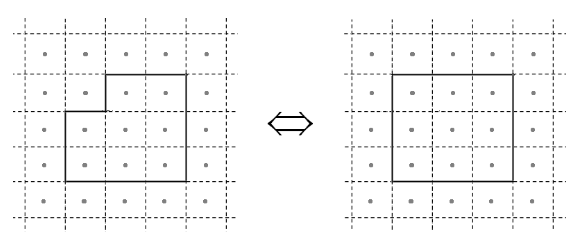
\includegraphics[width=0.7\textwidth]{Images/ising1.png}
  \caption{The lattice of dots represents the spin lattice, and the dashed
    lines are the interaction lattice. $L=12$ in both graphs, therefore both
    require the same energy, yet do not have the same number of spins flipped.}
    \label{fig:ising1}
\end{figure}
a boundary of length $L$ can be thought of as  an $L$ steps closed path
along the array's links. At each site, a choice of two directions is 
sufficient to guarantee a closed path\footnote{In the most general case, this
  number is four. However, when we exclude the possibility for back-tracking,
  we are left with three. Furthermore, as we are looking for an upper bound,
two is sufficient}.
\begin{figure}
  \centering
  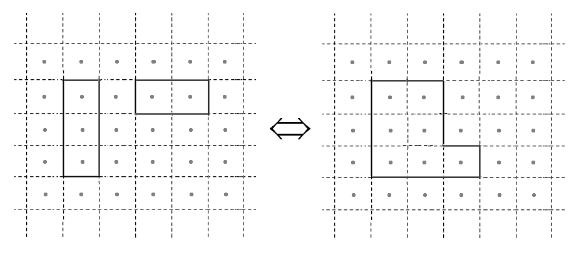
\includegraphics[width=0.7\textwidth]{Images/ising2.png}
  \caption{Same convention as above. Here $L=14$ in both cases, therefore
    both graphs are energetically equivalent, despite the different
  topologies.}
  \label{fig:ising2}
\end{figure}


There are then $2^L$ ways to realise a boundary given all
$L$, all topologies included, thus according to statistical mechanics
\begin{equation}
\Delta S = \log(2^L) = L\log(2)
\end{equation}
Combined with equation \eqref{eq:energyreq} we can express the variation in
freefree energy:
\begin{equation}
  \Delta F = \Delta E - T\Delta S = L(2J-T\log(2))
  \label{eq:freeenergyvar}
\end{equation}
At low temperature, where we can observe ferromagnetic behaviour, we can assume
stability of the creation of such boundaries, i.e $\Delta F \geq 0$. We can
obtain a first approximation to the critical temperature $T_c$, as approached
from below by plugging \eqref{eq:freeenergyvar} into the inequality
\begin{equation}
  T_c\approx \frac{2}{\log(2)}J\leq T
\end{equation}
which gives
\begin{equation}
  \boxed{
  T_C\approx 2.885J
}
\end{equation}
We can expand this argument for three dimensions if we suppose equation
\eqref{eq:energyreq} is still holds. On the other hand, we should only consider
$5^L$ ways to close a path in the cubic array. The same calculation lead to an
evaluation of the critical temperature of the 3d Ising model
\begin{equation}
  T_{C_{\mathrm{Ising}}} = \frac{2}{\log(5)}J\approx 1.243J
\end{equation}
This appears to be a lower temperature than in 2d. One is tempted to conclude
that thermal fluctuations are stronger than spin-spin interactions, as
dimensions increase. This approach, although na\"ive, has the power to
estimate a value of $T_C$ despite not being able to solve the model exactly.

\subsection{Kramers-Wannier duality}
The Kramers-Wannier duality is an extended symmetry in statistical physics. It
relates the free energy of a two-dimensional square-lattice Ising model at 
low temperature to that of another Ising model at high temperature. Kramers and
Wannier used this duality trick to find the exact location of the critical
point for the Ising model on the square lattice.

Let us investigate the behaviour of an $M\times M$ links square lattice\footnote{In
  the thermodynamical limit, when $M\rightarrow\infty$, the number of links and
  lattice points $N$ are indistinguishable. The calculation is made in the
interaction picture, and remains valid in the spin picture.}, in the absence
of an external field. To do so, we shall use the high, then low temperature
series expansion. We will mostly use geometrical arguments to consolidate the
expansion.
\subsubsection{High-Temperature Expansion}
Let us suppose the two coupling constants for the vertical and horizontal link-link
interaction to be identical $J_V =J_H = J$. If that is the case, we can write
the partition function 
\begin{equation}
  Z_M = \sum_s e^{J\sum_{\langle i,j\rangle}s_is_j + J\sum_{\langle
  i,k\rangle s_i s_k}}
\end{equation}
Using $K=\beta J$ and writing the exponent as a sum of hyperbolic functions,
we can rewrite $Z_M$ as follows,
\begin{equation}
  Z_M = (\cosh K)^{2M}\sum_s\left(\prod_{\langle i,j\rangle}
  (1+s_is_j\tanh K)\right)
\end{equation}
At high temperature, the system is in the  disordered phase. Because of the
unique dependence of $Z_M$ on $\tanh K$, let us observe the limit
$\lim_{T\rightarrow\infty}\tanh K = 0$. It is now natural to expand om the high 
temperature limit. In fact, expanding the product will produce $2^2M$ terms
that can be thought of graphically. Returning to figures
\ref{fig:ising1} and \ref{fig:ising2}, we can now rigorously construct them, and they
turn out to be highter order terms. The process is to represent each of the
three possible terms than can be produced: to every $s_is_j$ product there is
an associated vertical or horizontal link whereas to each factor 1 produced,
nothing is drawn. Repeating the process for all $2^2 M$ terms becomes
reminiscent of the random path created in the previous  section. In effect, it
corresponds to the geometrical quantity we implicitly used with Peierls'
argument, which outputs valid polygons given a length $L$:
\begin{equation}
  \Phi = \sum_P(\tanh K)^{p+q}
\end{equation}
where $p+q = L$ are the horizontal and vertical links drawn. Thus we have a
pre-expansion partition function written as
\begin{equation}
  Z_M = 2^N(\tanh K)M\Phi
\end{equation}
Now remains to sum over all polygons. Taking into account $s\in \mathbb{Z}_2$,
we can expect the conditions - listed in the previous section - for the
polygons to be valid to be naturally satisfied: in effect, the sum is null
unless it outputs an even $L$ per polygon.
\par The first term of the sum is clearly 1, corresponding to no domain wall.
The first non-trivial term is the smallest domain wall: a square of length
$L=4$, which can be placed anywhere on the lattice, hence occur $N$ times.
\subsubsection{Low-Temperature Expansion}
Not immediately obvious is that we can draw a correspondence between the
high-temperature limit in the interaction picture to the low temperature limit
in the spin picture. One can see that in the first case, the first term
corresponds
to no domain walls, indeed at $T=0$ all spins are aligned. One spin flipped is
bounded by the next term in the polygon expansion: the $L=4$ square.
\par Even without much details, this could be anticipated from the asymptotic
bound behaviour and odd parity of $\tanh K$. However, if we define a new 
variable $K^*$
\begin{equation}
  \tanh K = e^{-2K^*},
\end{equation}
we can rewrite the expansion of the partition function and arrive at the 
following relation
\begin{equation}
  \frac{Z(K^*)}{(e^{K^*})^N} = \frac{Z(K)}{(2\cosh^2 K)^N}
\end{equation}
By construction, we associated $K$ with the high temperature and $K^*$ with 
the low, such that they are inversely proportional to each other. Rearranging
both equations, we can make the duality finally obvious
\begin{tcolorbox}[title=Kramers-Wannier duality]
  \begin{equation}
    \frac{Z(K^*)}{\sinh^{N/2}(2K^*)} = \frac{Z(K)}{\sinh^{N/2}(2K)}
  \end{equation}
\end{tcolorbox}
The final argument is to suppose there are strictly two phases, hence one
critical temperature. If this is the case, then $K=K^*$, or
\begin{equation}
  \sinh(2K_C) = 1
\end{equation}
which gives the following result for the critical temperature of the 2d Ising
model
\begin{equation}
  T_C^{2d} = 2.269J
\end{equation}
\subsubsection{Exact Critical Temperature in 2d}
Now, with the low-high temperature self-duality made clear, we have acquired
the power to switch from one end of the temperature scale to the other, by
simply switching from the lattice to the interaction picture. This is
particularly useful when one calculation is hard or even impossible in one
limit, but feasible in the other limit.
\subsection{Note on Correspondence to String Theory}
Based purely on the dimensionsional arguments , one can draw parallels between
flipped spins and their domain walls, with particles and their world line.


\begin{table}[h]
  \begin{tabular}{|c|c|c|}
  \hline
  \textbf{Lattice Dimension} & \textbf{Domain Wall Dimension} & \textbf{String
  Theory Correspondant} \\ \hline
  2d & 1d & \begin{tabular}[c]{@{}c@{}}kink particle and its (0+1)-\\ d world
  line\end{tabular} \\ \hline
  3d & 2d & string and its (1+1)-d world line \\ \hline
  4d & 3d & 2-brane and its (2+1)-d world line \\ \hline
\end{tabular}
\caption{Lattice points and domain walls correspondence to String theory}
\end{table}
The high-low temperature Kramers-Wannier (self)-duality of the two-dimensional
Ising model is a particular example of the more general weak-strong
$S-duality$. Here the gauge group (and the dual group) is $\mathbb{Z}_2$, as
we saw earlier.
\subsection{Conclusion}
We have derived two exact solutions to the Ising model. In doing so, we have
discovered that at low dimensions the mean-field approximation leads to
erraneous results. As we increase in dimensions, and reach 4d, mean-field
theory is not only accurate, but the only way to provide insight into
our model.
\par Ironicall, the only thing the Ising model has failed to do is fulfil its
original intent and accurately reproduce ferromagnets. On the other hand, it
allowes us to explore exactly and analytically critical behaviours
that are insensitive to microscopic scales, hence the usefulness of
universality classes. It is indeed sufficient to study the Ising model as
a representative, to characterise the entire class. We had already noted
the appearance of the divergencies and the importance of the correlation
length, as hinting the need to introduce a quantum field language. Indeed,
using the correlation length as a variable, instead of the lattice length, in
other words coarse graining in the context of a renormalisation group
transformation, could be grounding for future work. Further investigation into
the conformality at the critical point, of the Ising model and all models
whose Hamiltonian is $\mathbb{Z}_2$ invariant at the same dimensions, would
provide elegant solutions.

